
\documentclass[a4paper,11pt]{article}
\usepackage[a4paper, margin=8em]{geometry}

% usa i pacchetti per la scrittura in italiano
\usepackage[french,italian]{babel}
\usepackage[T1]{fontenc}
\usepackage[utf8]{inputenc}
\frenchspacing 

% usa i pacchetti per la formattazione matematica
\usepackage{amsmath, amssymb, amsthm, amsfonts}

% usa altri pacchetti
\usepackage{gensymb}
\usepackage{hyperref}
\usepackage{standalone}

% imposta il titolo
\title{Appunti Fondamenti di Automatica}
\author{Luca Seggiani}
\date{2025}

% disegni
\usepackage{pgfplots}
\pgfplotsset{width=10cm,compat=1.9}

% imposta lo stile
% usa helvetica
\usepackage[scaled]{helvet}
% usa palatino
\usepackage{palatino}
% usa un font monospazio guardabile
\usepackage{lmodern}

% tikz in sans
\tikzset{every picture/.style={/utils/exec={\sffamily}}}

\renewcommand{\rmdefault}{ppl}
\renewcommand{\sfdefault}{phv}
\renewcommand{\ttdefault}{lmtt}

% circuiti
\usepackage{circuitikz}
\usetikzlibrary{babel}

% disponi il titolo
\makeatletter
\renewcommand{\maketitle} {
	\begin{center} 
		\begin{minipage}[t]{.8\textwidth}
			\textsf{\huge\bfseries \@title} 
		\end{minipage}%
		\begin{minipage}[t]{.2\textwidth}
			\raggedleft \vspace{-1.65em}
			\textsf{\small \@author} \vfill
			\textsf{\small \@date}
		\end{minipage}
		\par
	\end{center}

	\thispagestyle{empty}
	\pagestyle{fancy}
}
\makeatother

% disponi teoremi
\usepackage{tcolorbox}
\newtcolorbox[auto counter, number within=section]{theorem}[2][]{%
	colback=blue!10, 
	colframe=blue!40!black, 
	sharp corners=northwest,
	fonttitle=\sffamily\bfseries, 
	title=Teorema~\thetcbcounter: #2, 
	#1
}

% disponi definizioni
\newtcolorbox[auto counter, number within=section]{definition}[2][]{%
	colback=red!10,
	colframe=red!40!black,
	sharp corners=northwest,
	fonttitle=\sffamily\bfseries,
	title=Definizione~\thetcbcounter: #2,
	#1
}

% disponi problemi
\newtcolorbox[auto counter, number within=section]{problem}[2][]{%
	colback=green!10,
	colframe=green!40!black,
	sharp corners=northwest,
	fonttitle=\sffamily\bfseries,
	title=Problema~\thetcbcounter: #2,
	#1
}

% disponi codice
\usepackage{listings}
\usepackage[table]{xcolor}

\lstdefinestyle{codestyle}{
		backgroundcolor=\color{black!5}, 
		commentstyle=\color{codegreen},
		keywordstyle=\bfseries\color{magenta},
		numberstyle=\sffamily\tiny\color{black!60},
		stringstyle=\color{green!50!black},
		basicstyle=\ttfamily\footnotesize,
		breakatwhitespace=false,         
		breaklines=true,                 
		captionpos=b,                    
		keepspaces=true,                 
		numbers=left,                    
		numbersep=5pt,                  
		showspaces=false,                
		showstringspaces=false,
		showtabs=false,                  
		tabsize=2
}

\lstdefinestyle{shellstyle}{
		backgroundcolor=\color{black!5}, 
		basicstyle=\ttfamily\footnotesize\color{black}, 
		commentstyle=\color{black}, 
		keywordstyle=\color{black},
		numberstyle=\color{black!5},
		stringstyle=\color{black}, 
		showspaces=false,
		showstringspaces=false, 
		showtabs=false, 
		tabsize=2, 
		numbers=none, 
		breaklines=true
}

\lstdefinelanguage{javascript}{
	keywords={typeof, new, true, false, catch, function, return, null, catch, switch, var, if, in, while, do, else, case, break},
	keywordstyle=\color{blue}\bfseries,
	ndkeywords={class, export, boolean, throw, implements, import, this},
	ndkeywordstyle=\color{darkgray}\bfseries,
	identifierstyle=\color{black},
	sensitive=false,
	comment=[l]{//},
	morecomment=[s]{/*}{*/},
	commentstyle=\color{purple}\ttfamily,
	stringstyle=\color{red}\ttfamily,
	morestring=[b]',
	morestring=[b]"
}

% disponi sezioni
\usepackage{titlesec}

\titleformat{\section}
	{\sffamily\Large\bfseries} 
	{\thesection}{1em}{} 
\titleformat{\subsection}
	{\sffamily\large\bfseries}   
	{\thesubsection}{1em}{} 
\titleformat{\subsubsection}
	{\sffamily\normalsize\bfseries} 
	{\thesubsubsection}{1em}{}

% disponi alberi
\usepackage{forest}

\forestset{
	rectstyle/.style={
		for tree={rectangle,draw,font=\large\sffamily}
	},
	roundstyle/.style={
		for tree={circle,draw,font=\large}
	}
}

% disponi algoritmi
\usepackage{algorithm}
\usepackage{algorithmic}
\makeatletter
\renewcommand{\ALG@name}{Algoritmo}
\makeatother

% disponi numeri di pagina
\usepackage{fancyhdr}
\fancyhf{} 
\fancyfoot[L]{\sffamily{\thepage}}

\makeatletter
\fancyhead[L]{\raisebox{1ex}[0pt][0pt]{\sffamily{\@title \ \@date}}} 
\fancyhead[R]{\raisebox{1ex}[0pt][0pt]{\sffamily{\@author}}}
\makeatother

\begin{document}

% sezione (data)
\section{Lezione del 01-04-25}

% stili pagina
\thispagestyle{empty}
\pagestyle{fancy}

% testo
\noindent
\begin{minipage}{\textwidth}
\subsection{Dettaglio sulla risposta dei sistemi sottosmorzati}
Vediamo in particolare alcune grandezze di interesse nel caso di sistemi di secondo grado sottosmorzati:

\par\bigskip

\begin{center}
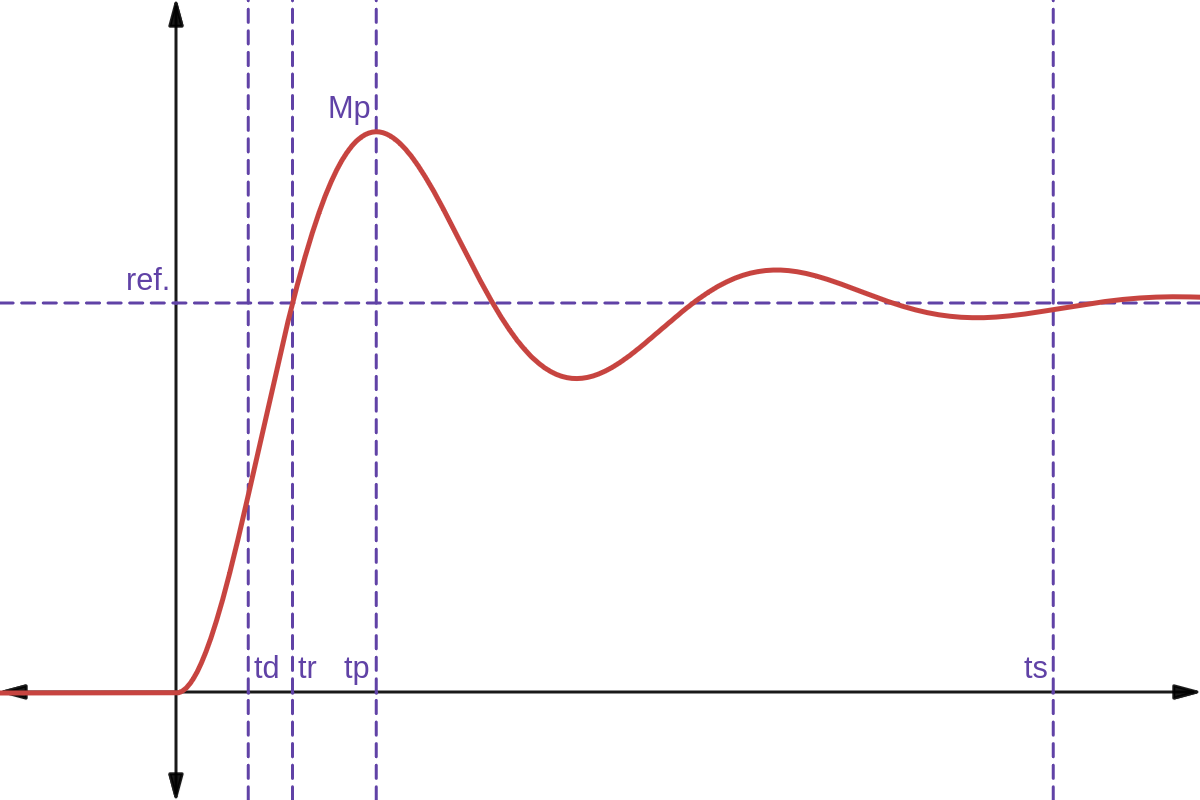
\includegraphics[scale=0.29]{../figures/damped_oscillator.png}
\end{center}
\end{minipage}

\par\bigskip

Abbiamo che una caratteristica del loro comportamento è la \textbf{sovraelongazione} al di sopra del valore bersaglio.
Chiamiamo quindi $M_p$ la \textit{massima sovraelongazione} sopra il livello di riferimento, e $t_p$ l'istante temporale in cui questa viene raggiunta.
Avremo poi il tempo $t_r$ \textit{di salita}, il momento in cui viene toccato per la prima volta il valore bersaglio, e il tempo $t_d$ \textit{di ritardo}, che viene impiegato a raggiungere il 50\% del valore bersaglio.
Infine, per valutare il comportamento oscillante dopo il transiente iniziale, consideriamo il tempo $t_s$ \textit{di assestamento}, oltre il quale il segnale resta in una certa (piccola) percentuale del valore bersaglio.

\noindent
\begin{minipage}{\textwidth}
Vediamo il comportamento generale dei sistemi di questo tipo al variare del valore di smorzamento $\xi = \frac{a_1}{2 \sqrt{a_0 a_2}}$:

\par\bigskip

\begin{center}
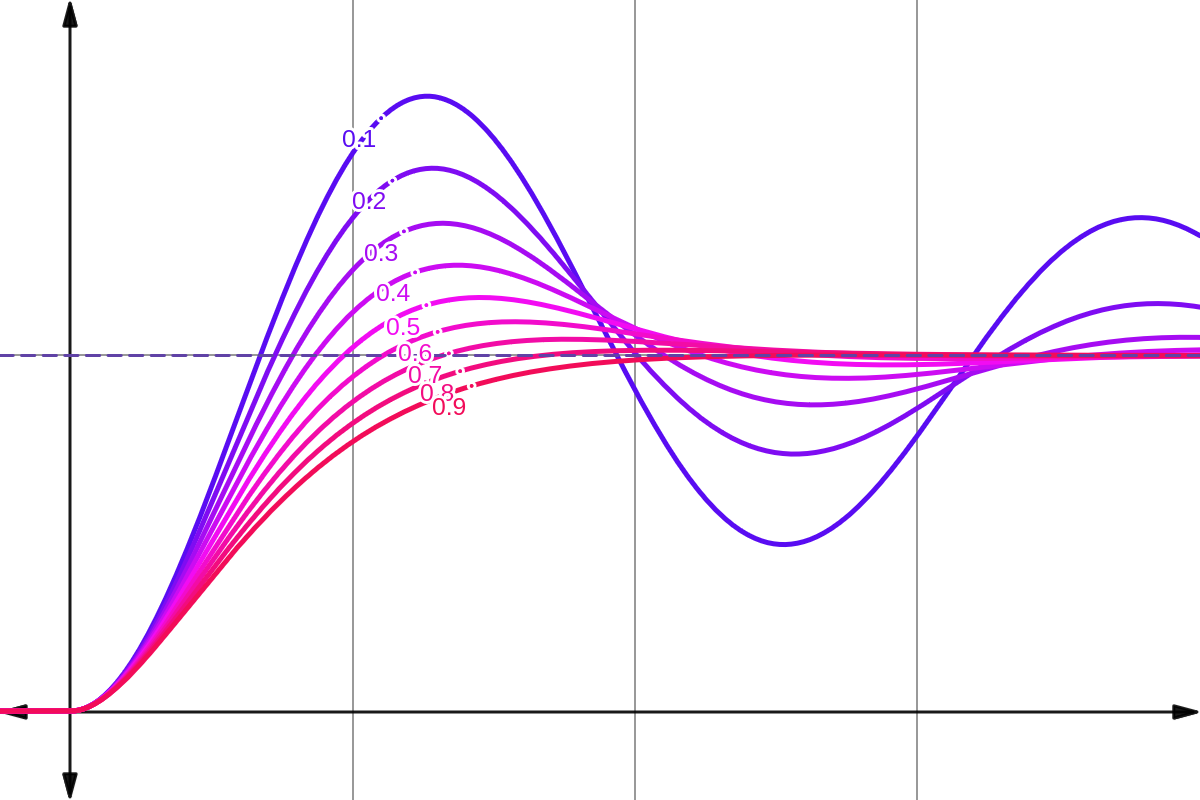
\includegraphics[scale=0.29]{../figures/damping_values.png}
\end{center}
\end{minipage}

\par\bigskip

Da dove notiamo che a valori di smorzamento maggiori si ha minore sovraelongamneto, ma anche maggiore tempo di salita.

Notiamo che possiamo considerare gli stessi parametri considerati sui sistemi sottosmorzati anche per sistemi criticamente smorzati o sovrasmorzati: infatti, se non per il tempo e per il punto di sovraelengazione, questi avranno valori ben definiti per qualsiasi sistema del second'ordine.

Tornando al dettaglio dei sistemi sottosmorzati, possiamo trovare le seguenti formule:
\begin{itemize}
	\item \textbf{Sovraelongazione:} si ha il picco in:
		$$
			S\% \ (M_p) \ = 100 e^{- \frac{\xi \pi}{\sqrt{1 - \xi^2}}}
		$$
		raggiunto all'istante:
		$$
			t_p = \frac{\pi}{\omega \sqrt{1 - \xi^2}}
		$$
	\item \textbf{Periodo di oscillazione:} possiamo considerare anche il periodo (e quindi la frequenza) delle oscillazioni, considerando il polo in $\beta$:
		$$
			T_o = \frac{2\pi}{\omega \sqrt{1 - x^2}}
		$$
		$$
			f_o = \frac{\omega \sqrt{1 - x^2}}{2\pi} 
		$$
	\item \textbf{Tempo di assestamento:} consideriamo questo come:
		$$
		t_s \approx -\frac{1}{\xi \omega} \ln(0.05)
		$$
	\item \textbf{Tempo di salita} consideriamo infine questo, con molta approssimazione, come:
		$$
		t_r \approx \frac{1.8}{\omega}
		$$
\end{itemize}

\subsubsection{Derivazione alternativa della funzione sottosmorzata}
Avevamo ricavato l'espressione:
$$
y(t) = \frac{b_0}{a_0} \left( 1 - e{\alpha t} \cos(\beta t) + \frac{\alpha}{\beta} e^{\alpha t} e^{\alpha t} \sin(\beta t) \right) \cdot H(t)
$$
per i sistemi del second'ordine sottosmorzati.
Vediamo come si può svolgere una derivazione, attraverso Laplace, per arrivare alla forma (equivalente):
$$
y(t) = G(0) \cdot \left( 1 - e^{-\xi \omega t} \cos\left(\omega \sqrt{1 - \xi ^2} \cdot t \right) - \frac{\xi}{\sqrt{1 - \xi^2}} e^{-\xi \omega t} \sin\left( \omega \sqrt{1 - \xi^2} \cdot t \right) \right)
$$
vediamo come questa evidenzia la dipendenza dal guadagno $G(0)$, e dai valori di pulsazione naturale $\omega$ e smorzamento $\xi$.

# fallo

Il lato destro dell'espressione trovata si può chiaramente riscrivere nella forma più concisa $ke^{-\sigma t} \sin(\omega t + \alpha)$. 
Usiamo allora le formule di traduzione in forma sinusoidale, di cui una dimostrazione nel caso cosinusoidale si trova a \url{https://github.com/seggiani-luca/appunti-fis/blob/main/master/master.pdf}:
\[
	c_1 \sin{\omega t} + c_2 \cos{\omega t}
	\Leftrightarrow
	k \sin(\omega t + \alpha)
\]
con:
\[
	\begin{cases}
		k 	= \sqrt{c_1^2 + c_2^2} \\ 
		\alpha = \tan^{-1}(\frac{c1}{c2})
	\end{cases}
\]

che darà quindi:
$$
y(t) = G(0) \cdot \left( 1 - e^{-\xi \omega t} \sqrt{1 + \frac{\xi^2}{1 + \xi^2}} \sin\left( \omega \sqrt{1 - \xi^2} \cdot t + \tan^{-1} \left( \frac{\sqrt{1 - \xi^2}}{\xi} \right) \right) \right) 
$$

\subsection{Stabilità nel modello a funzione di trasferimento}
Abbiamo lavorato finora col modello a funzione di trasferimento, definita come:
$$
G(s) = \frac{\sum_{i = 0}^m b_i s^i}{\sum_{i = 0}^n a_i s^i} = \frac{ b_m (s - z_1) (s - z_2) ... (s - z_m) }{ a_n (s - p_1) (s - p_2) ... (s - p_n) }
$$
con $z_i$ gli $m$ \textit{zeri}, $p_i$ gli $n$ \textit{poli}, e $n > m$.

Di questa avevamo individuato le due forme:
\begin{itemize}
	\item \textbf{Forma di Evans:} evidenzia poli e zeri:
		$$
G(s) = \frac{\sum_{i = 0}^m b_i s^i}{\sum_{i = 0}^n a_i s^i} = \frac{ b_m (s - z_1) (s - z_2) ... (s - z_m) }{ a_n (s - p_1) (s - p_2) ... (s - p_n) }
		$$
	\item \textbf{Forma di Bode:} evidenzia le costanti tempo: 
		$$
G(s) = K \frac{ (\tau_a s + 1) (\tau_b s + 1) ... (\tau_i s + 1) }{ (\tau_1 s + 1) (\tau_2 s + 1) ... (\tau_n s + 1) }
		$$
\end{itemize}

Definiamo quindi formalmente \textbf{poli}:
\begin{definition}{Polo}
	Un polo $a_i$ di una funzione di trasferimento $G(s)$ è un valore di $s$ per cui $G(s)$ tende ad infinito:
	$$
	F(s) = \frac{g(s)}{\prod_{i = 1}^x (s - a_i)^n_i}
	$$
	con $n_i$ ordine del polo.
\end{definition}
e \textbf{zeri}:
\begin{definition}{Zeri}
	Uno zero $a_i$ di una funzione di trasferimento $G(s)$ è un valore di $s$ per cui $G(s)$ tende a zero: 
	$$
	F(s) = \frac{\prod_{i = 1}^x (s - a_i)^m_i}{g(s)}
	$$
	con $m_i$ ordine dello zero.
\end{definition}

Quello che ci interesserà nella valutazione della \textbf{stabilità} dei sistemi sarà la posizione dei poli nel piano complesso.
In particolare, come avevamo detto per i modi nel modello a variabili di stato, poli a componente \textit{reale negativa} danno \textbf{stabilità asintotica}, poli a componente \textit{reale nulla} danno \textbf{stabilità marginale}, e poli a componente \textit{reale positiva} dano \textbf{instabilità}.
Inoltre la componente \textit{complessa} dà informazioni sull'oscillazione del sistema, con \textbf{oscillazioni smorzate} a componente \textit{complessa e reale non nulle}, e \textbf{oscillazioni continue} a componente \textit{reale nulla}.

Gli zeri, invece, non hanno effetto sulla stabilità.
Gli zeri a parte reale positiva hanno invece l'effetto di \textit{invertire} la risposta al gradino, almeno sul breve termine.

\subsubsection{Conversione da spazio di stato a funzione di trasferimento}
Dovrebbe ormai essere chiaro che lo spazio di stato e la funzione di trasferimento rappresentano due modi di modelizzare lo stesso tipo di fenomeni.
Vediamo quindi come passare dall'uno all'altro.

Partiamo dal modello a variabili di stato:
\[
	\begin{cases}
		x' = Ax + Bu \\
		y = Cx + Du
	\end{cases}
\]

Assumendo condizioni iniziali nulle, si ha:
\[
	\begin{cases}
		s X(s) = A X(s) + B U(s)  \\ 
		Y(s) = C X(s) + D U(s) 
	\end{cases} \implies
	\begin{cases}
		X(s) = (sI - A)^{-1} B U(s) \\
		Y(s) = \left( C(sI - A)^{-1} B + D \right) U(s)
	\end{cases}
\]
notando che $X, U$ sono vettori e $A, B$ matrici.

Si trova quindi la funzione di trasferimento:
$$
G(s) = \frac{Y(s)}{U(s)} = C(sI - A)^{-1} B + D
$$

\subsubsection{Forme canoniche di controllo}
Esistono un numero infinito di possibili modelli in spazio di stato che forniscono la stessa dinamica ingresso/uscita.

Aiuta avere alcune strutture standardizzate dei modelli in spazio di stato: queste sono le cosiddette forme canoniche.
Data la funzione di trasferimento di un sistema, è possibile ottenere ciascuna delle forme canoniche.
Data una particolare forma canonica, è poi possibile trasformarla in qualsiasi altra forma.

Consideriamo ad esempio il sistema definito da:
$$
y^{(n)} + a_1 y^{(n - 1)} + ... + a_{n - 1}y' + a_n y = b_0 u^{(n)} + b_1 u^{(n - 1)} + ... + b_{n - 1} u' + b_nu
$$

Prendendo la trasformata di Laplace da entrambi i lati si ha:
$$
Y(s) \left( s^n + a_1 s^{n - 1} + ... + a_{n - 1} s + a_n \right) = U(s) \left( b_0 s^n + b_1 s^{n - 1} + ... + b_{n - 1} s + b_n \right)
$$
da cui la funzione di trasferimento:
$$
G(s) = \frac{Y(s)}{U(s)} = \frac{ b_0 s^n + b_1 s^{n - 1} + ... + b_{n - 1} s + b_n}{s^n + a_1 s^{n - 1} + ... + a_{n - 1} s + a_n }
$$

Mentre avevamo già visto come la stessa forma in variabili di stato aveva l'aspetto:
\[
	\begin{cases}	
x' = \left(\begin{array}{@{}c | cccc@{}}
	0 & 1 & 0 & ... & 0 \\
	0 & 0 & 1 & ... & 0 \\
	... & ... & ... & ... & ... \\
	0 & 0 & 0 & ... & 1 \\
	\hline
	-a & ... & ... & ... & -a_{n - 1}
\end{array}\right)
x + \begin{pmatrix}
0 \\
... \\
0 \\
1
\end{pmatrix} u \\ 
y = \begin{pmatrix}
	b_0 - b_n a_0 & ... & b_{n - 1} - b_n a_{n - 1}	
\end{pmatrix} x + \begin{pmatrix}
b_n
\end{pmatrix} u
	\end{cases}
\]

# confronta

\end{document}
